\part*{}

\chapter{Schlussbetrachtungen} % (fold)
\label{cha:schlussbetrachtungen}

\begin{figure}[htbp]
	\centering
		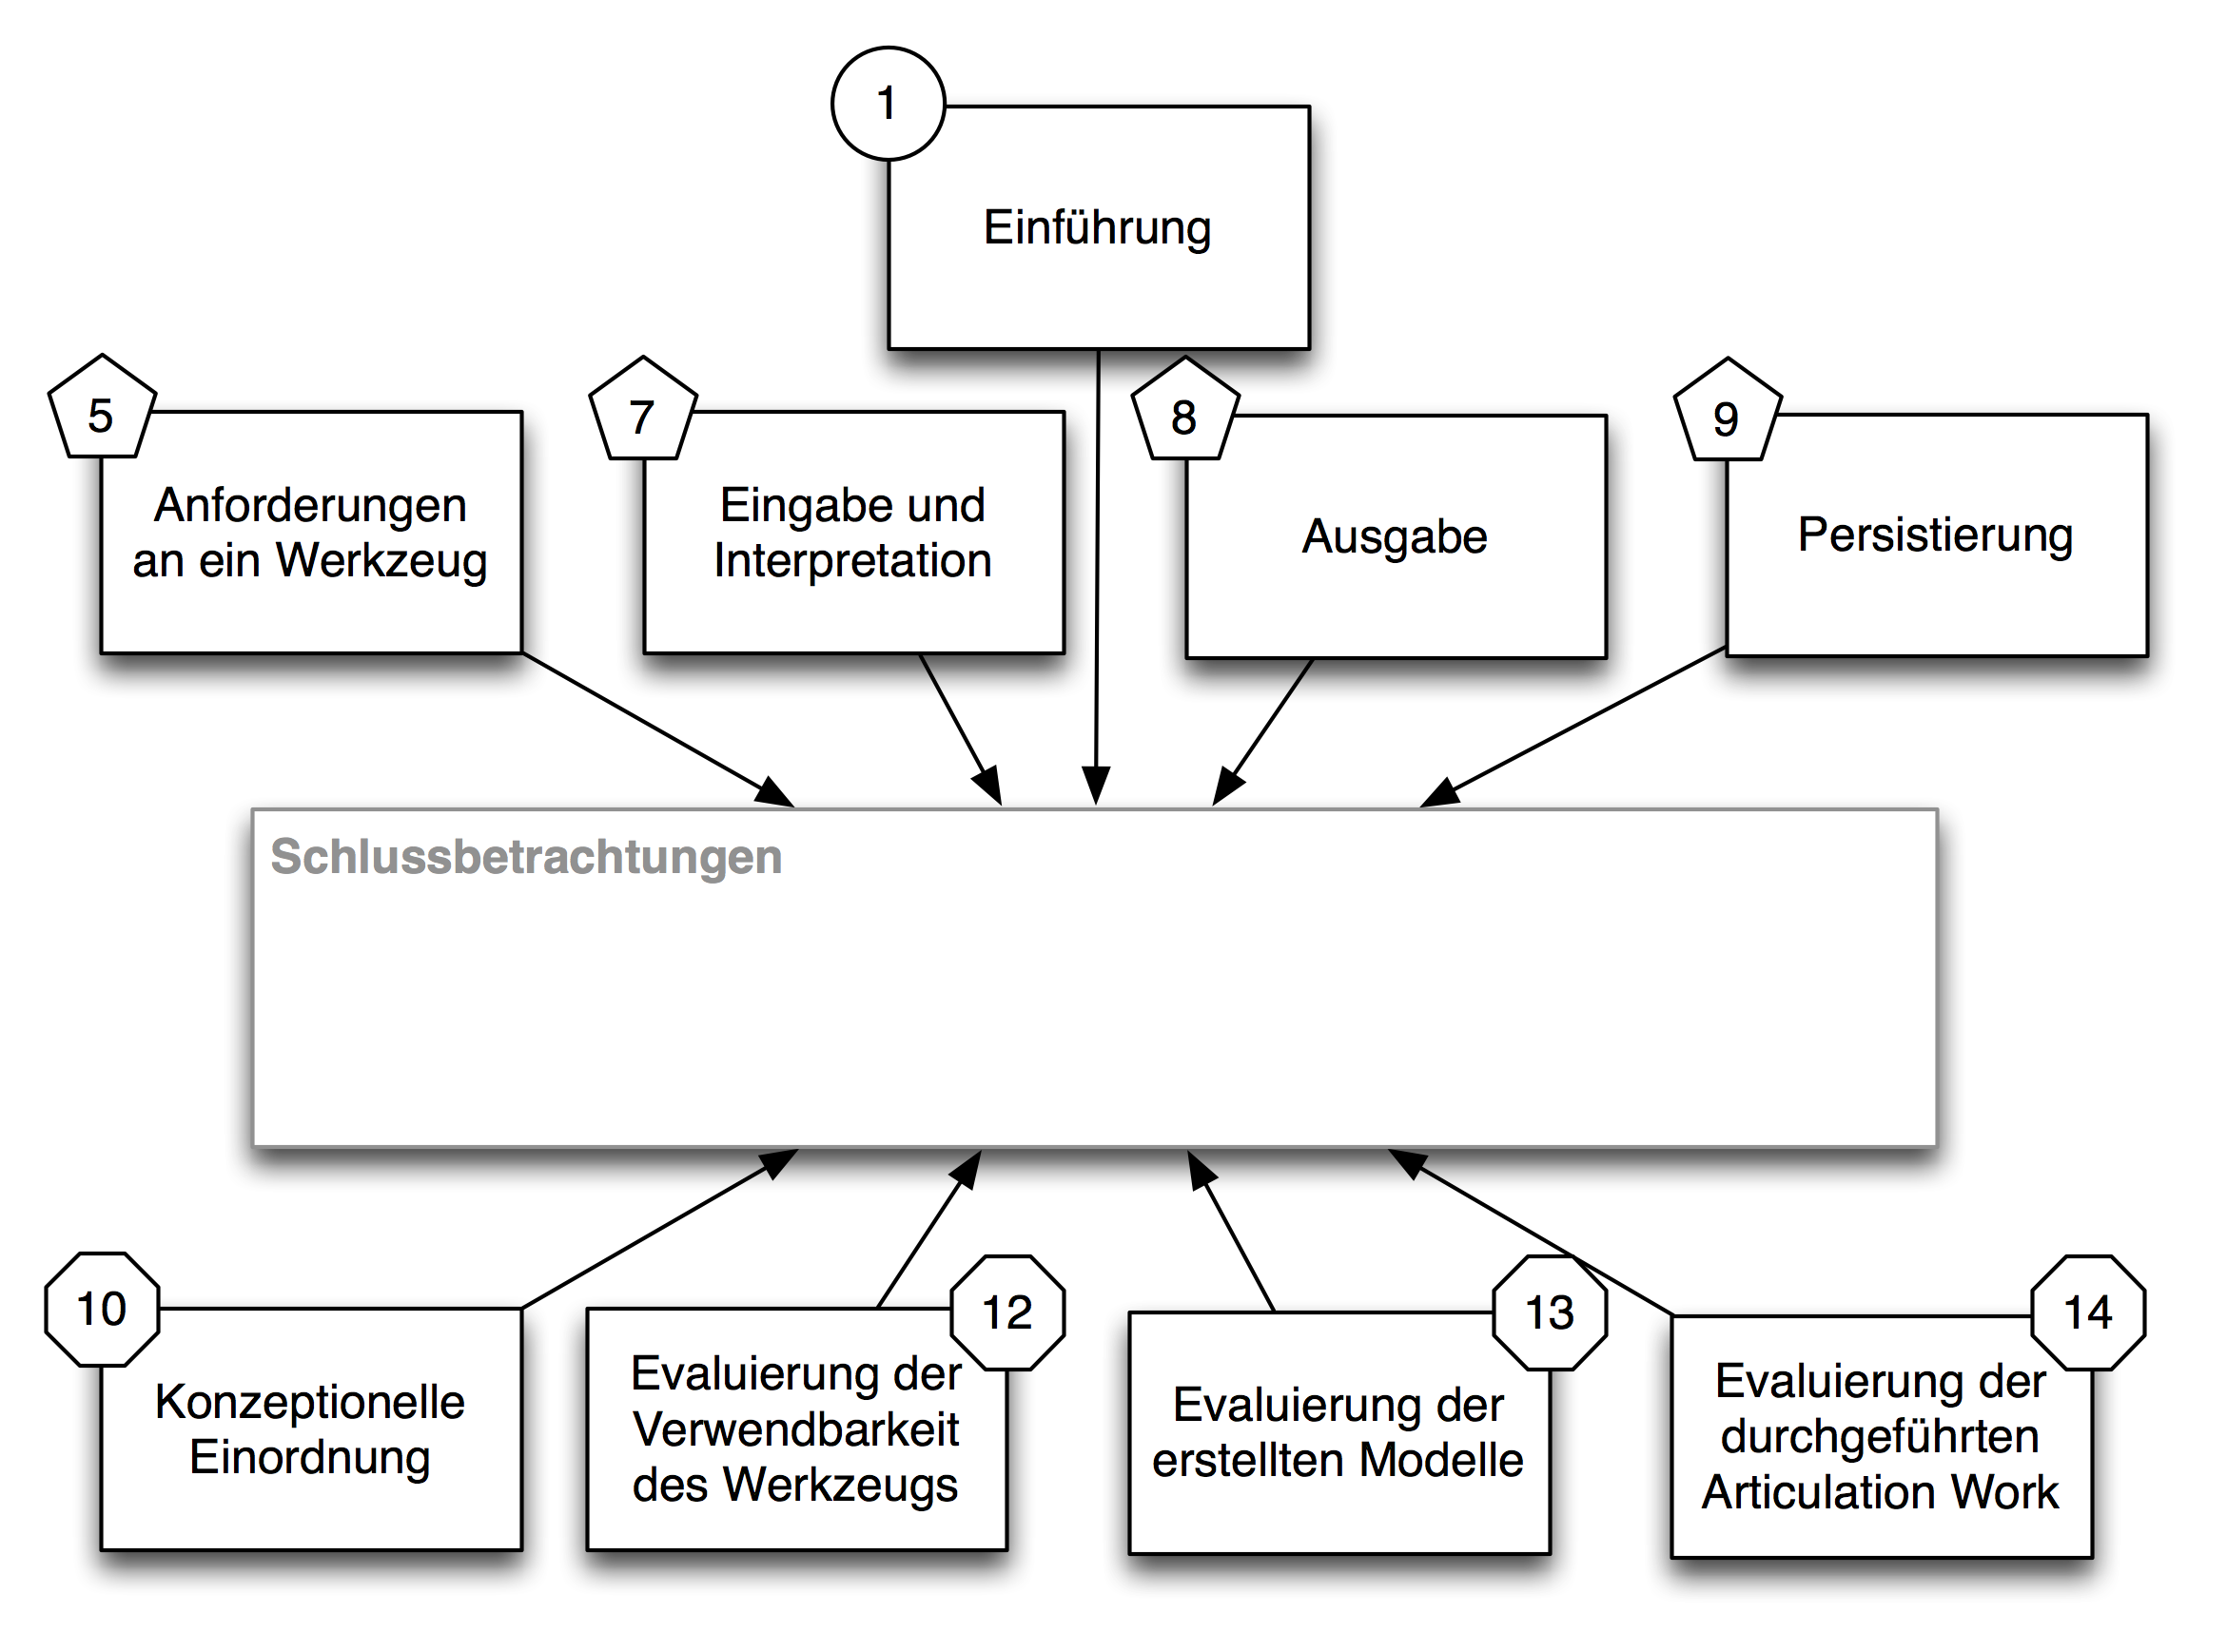
\includegraphics[scale=0.6]{img/Kontextgrafiken/k15.png}
	\caption{Kapitel „Schussbetrachtungen“ im Gesamtzusammenhang}
	\label{fig:img_Kontextgrafiken_k15}
\end{figure}

\section{Überblick über den Gesamtzusammenhang} % (fold)
\label{sec:überblick_über_den_gesamtzusammenhang}

\begin{figure}[htbp]
	\centering
		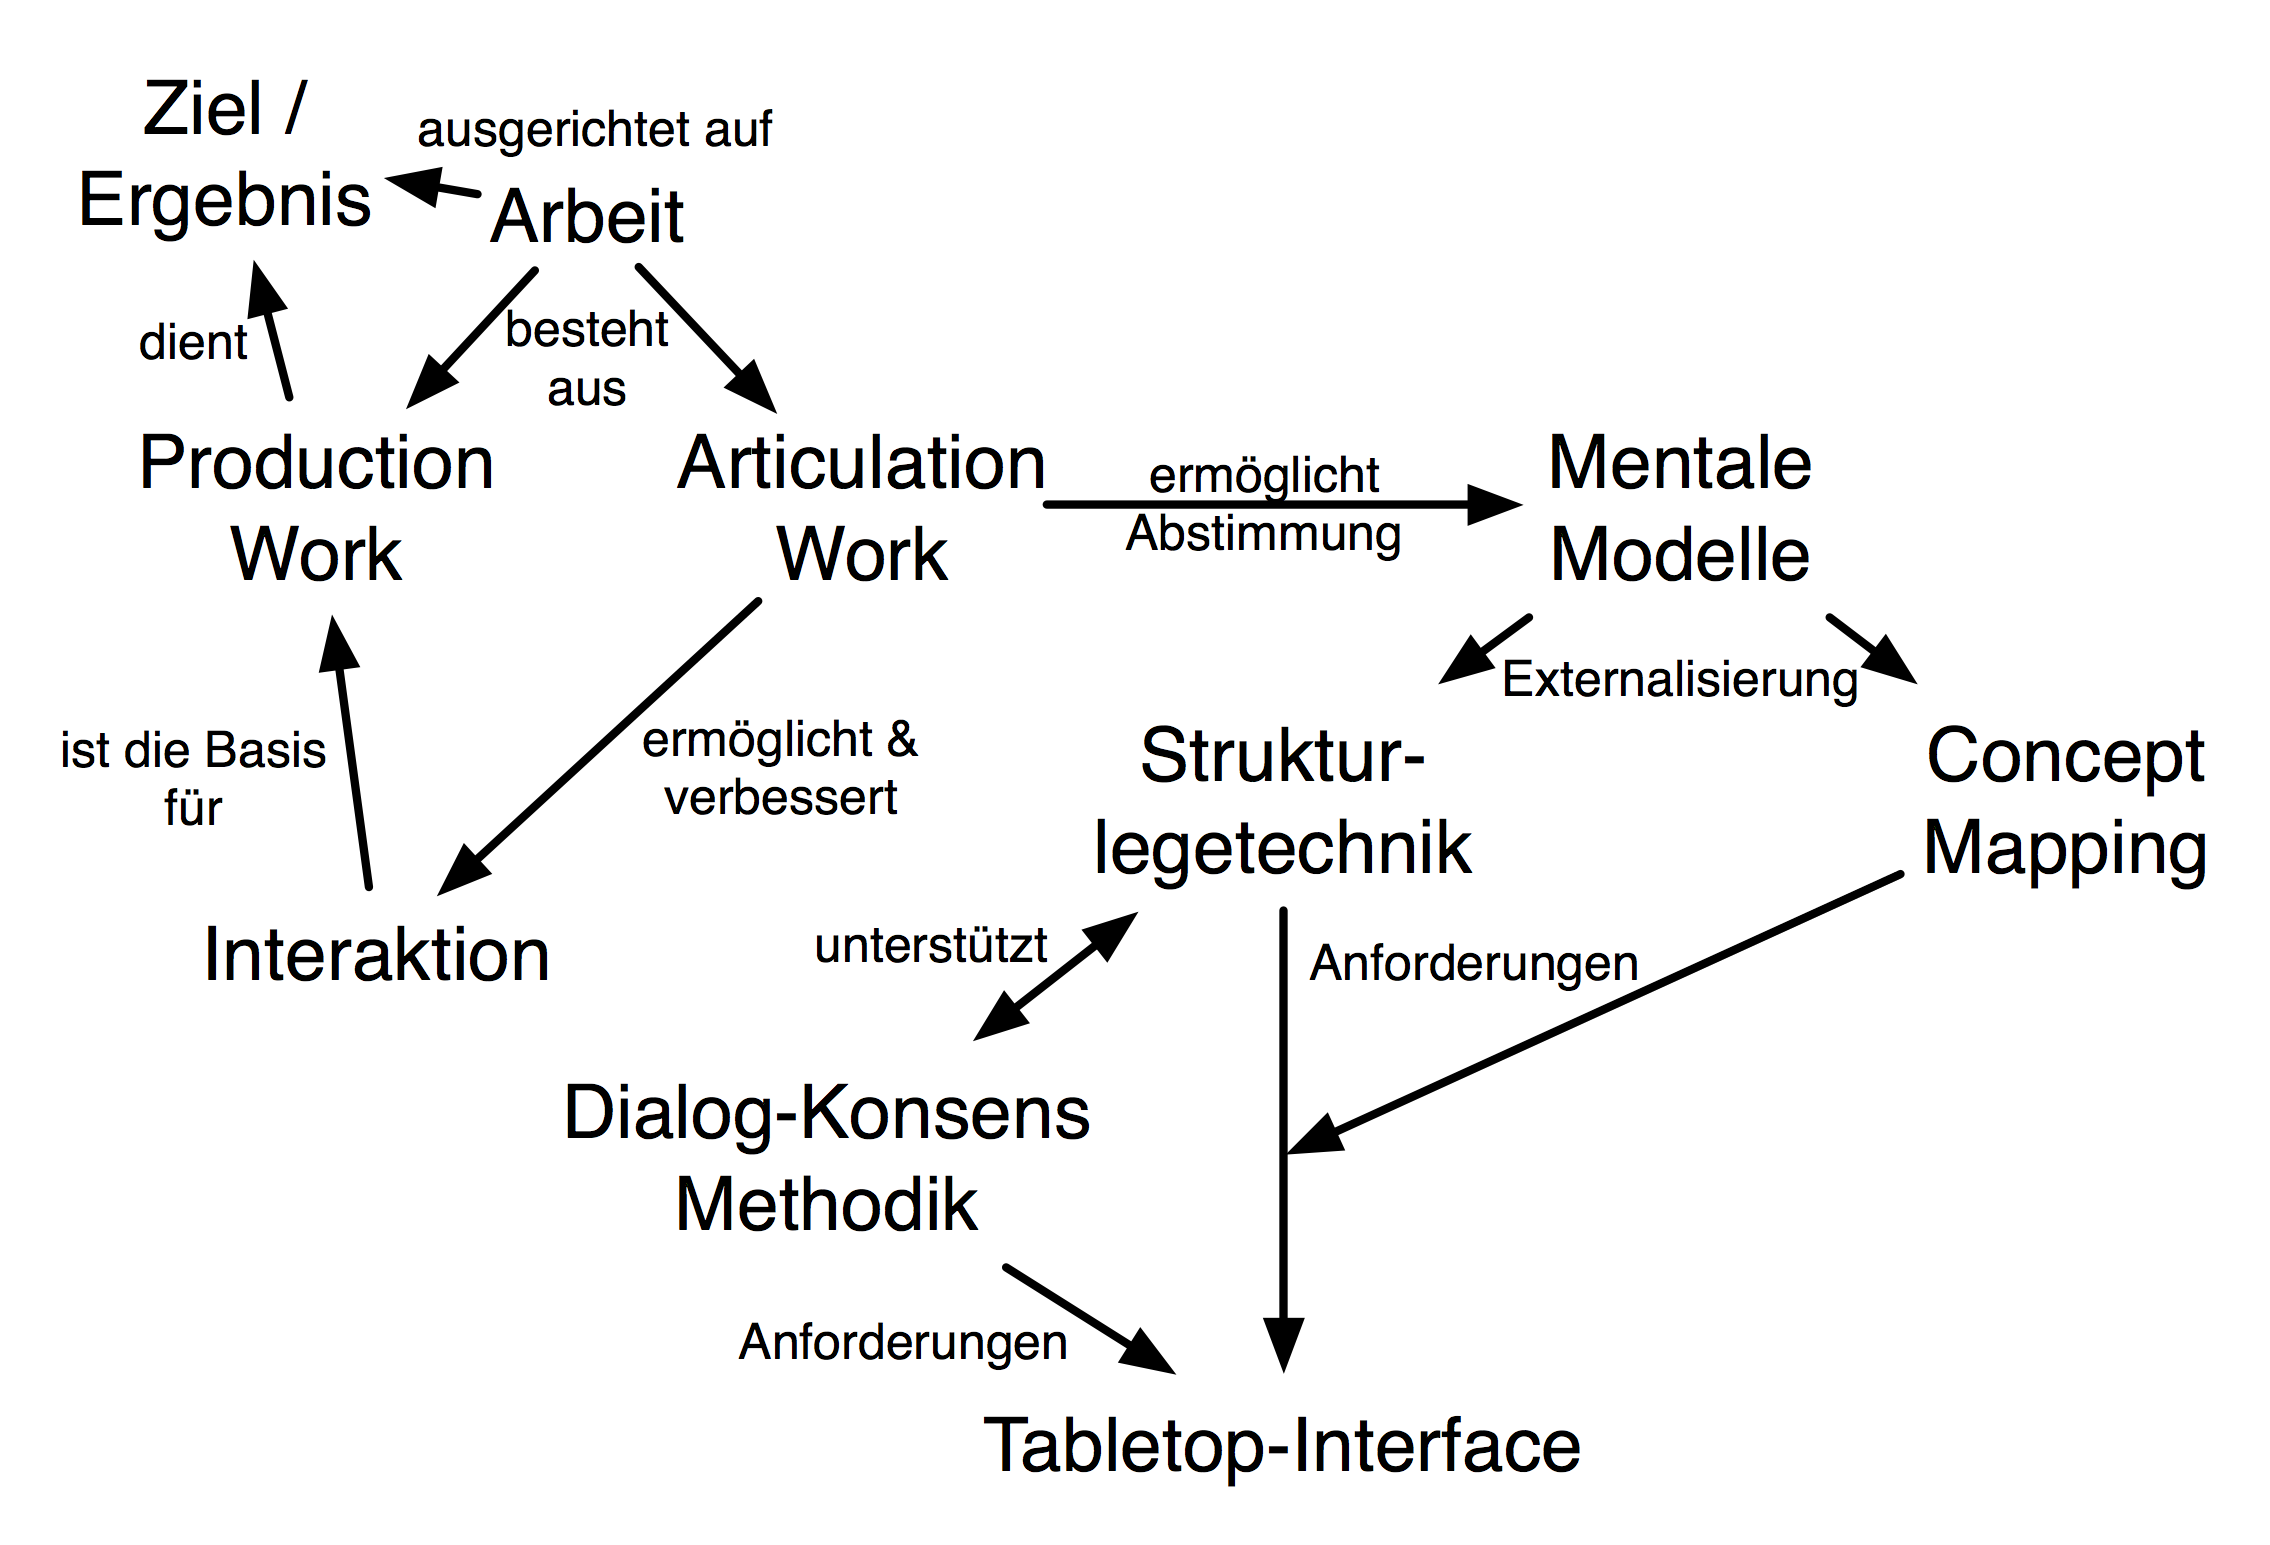
\includegraphics[width=10cm]{img/Schlussbetrachtungen/ArbeitInteraktionMentaleModelleTabletop.png}
	\caption{Gesamtzusammenhang der in dieser Arbeit verwendeten Konzepte}
	\label{fig:img_Schlussbetrachtungen_ArbeitInteraktionMentaleModelleTabletop}
\end{figure}

evtl. noch zweite Grafik, die die Kapitel der Arbeit in diese Struktur einordnet.

% section überblick_über_den_gesamtzusammenhang (end)

\section{Zusammenfassung der Evaluierung}

In diesem Abschnitt wird die in den Kapiteln \ref{cha:eval_ueberblick}, \ref{cha:eval_werkzeug}, \ref{cha:eval_modell} und \ref{cha:eval_aw} beschriebene empirische Untersuchung zusammengefasst und den Ergebnissen der konzeptuellen Einordnung in Kapitel \ref{cha:konzeptionelle_evaluierung} gegenübergestellt.

\subsection{Empirische Untersuchung}

In der empirischen Untersuchung waren folgende in Kapitel \ref{cha:eval_ueberblick} formulierte Untersuchungsfragen zu beantworten:

\begin{itemize}
 \item Sind das Werkzeug und dessen Komponenten verständlich und wie intendiert einsetzbar? (Aspekt: Werkzeug)
 \item Erlauben Werkzeug und Methode die Abbildung semantisch offener diagrammatischer Modelle? (Aspekt: Modell)
 \item Unterstützen Werkzeug und Methode Articulation Work? (Aspekt: Articulation Work)
\end{itemize}

Jede dieser Fragen wurde in einem separaten Kapitel bearbeitet. Die Untersuchungsfragen wurden in Hypothese konkretisiert, die den jeweiligen Untersuchungsgegenstand in Bezug zu den aus den konzeptuellen Grundlagen abgeleiteten Anforderungen an die Unterstützung von Articulation Work stellen.

Bei der Betrachtung der ersten Untersuchungsfrage wurden 8 Hypothesen geprüft, die die grundlegenden Anforderungen an das Werkzeug abdecken bzw. die Verständlichkeit und Verwendbarkeit der implementierten Funktionen testen. Insgesamt scheint das Werkzeug für den intendierten Verwendungszweck -- der kooperativen Erstellung von diagrammatischen Modellen -- in unterschiedlichen Anwendungsgebieten einsetzbar zu sein. Stabilitätsprobleme in der technischen Umsetzung führten jedoch in den ersten Phasen der Evaluierung zu Behinderungen bei der Modellbildung, was jedoch durch nachträglich durchgeführte Verbesserungen weitgehend kompensiert werden konnte. Herausforderungen zeigten sich im Interaktionsdesign der über die Kernfunktionalität hinausgehenden Funktionen zur Unterstützung des Modellbildungsprozesses. Die aus der Literatur begründbare Funktion zur Verfolgung der Modellierungshistorie und der Wiederherstellung vergangener Modellzustände wurde kaum genutzt. Auch die Verwendung der Funktion zur Entfernung von unerwünschten Verbindern im Modell war den Benutzern in der ersten Version unverständlich. Dieses Problem konnte durch ein Redesign des entsprechenden Teilwerkzeugs und dessen Bedienung beseitigt werden. Generell scheint das Werkzeug schnell erlenbar zu sein, so dass die Anzahl der Fehlbedienungen durch Missverständnisse bereits bei der zweiten Anwendung des Werkzeugs durch die Benutzer massiv reduziert bzw. nicht mehr vorhanden war. Die oben formulierte Frage kann also mit Vorbehalten positiv beantwortet werden. Generell scheint das Werkzeug wie intendiert einsetzbar und zum Großteil verständlich zu sein, einige Komponenten weisen jedoch Defizite in der Verständlichkeit auf.

Frage 2

Frage 3

\subsection{Gegenüberstellung der empirischen und konzeptuellen Untersuchung}

noch offen

\section{Erfüllung der Anforderungen an das Werkzeug}

In diesem Abschnitt werden die in Kapitel \ref{cha:anforderungen} formulierten Anforderungen an das Werkzeug hinsichtlich ihrer Erfüllung betrachtet. Die Beurteilung der Erfüllung erfolgt anhand der empirischen Ergebnisse, die in den Kapiteln \ref{cha:eval_werkzeug}, \ref{cha:eval_modell} und \ref{cha:eval_aw} beschrieben wurden.

Anforderung \ref{anf:physische_abbildung_legen_beliebiger_diagrammatischer_modelle} (Physische Abbildung beliebiger diagrammatischer Modelle) wurde in den Hypothesen \ref{hyp:diagmodelle}, \ref{hyp:behinderung} und \ref{hyp:gewöhnung} untersucht. Die grundlegende Abbildung diagrammatischer Modelle mit dem Werkzeug ist ohne Einschränkung der Anwendungsdomäne möglich. Bei der Untersuchung des Prozesses der physischen Abbildung der Modelle konnten in den ersten durchgeführten Evaluierungsblöcken behindernde Aspekte identifiziert werden. Diese hatten Einfluss auf die Abbildung der Modelle, insbesondere die Möglichkeit des Einsatzes von Verbindern im Modell wurde nur eingeschränkt wahrgenommen. Nach Überarbeitungen des Interaktionsdesigns und der Implementierung mehrerer Maßnahmen zur Steigerung der Robustheit gegenüber Fehlerkennungen von Benutzereingaben konnten die als behindernd wahrgenommenen Faktoren reduziert werden. Bei mehrmaliger Verwendung des Werkzeugs zeigt sich eine Verbesserung des Umgangs mit den zur Verfügung gestellten Ausdrucksmöglichkeiten und eine stärke Fokussierung auf den zu repräsentierenden Sachverhalt. Insgesamt kann diese Anforderung als erfüllt angesehen werden.

\todo Anforderung \ref{anf:unterstützung_der_iterativen_aushandlung_des_modells} (Unterstützung der iterativen Aushandlung des Modells) wurde in der Hypothese \ref{hyp:abstimmung} untersucht.

Anforderung \ref{anf:ermöglichung_experimenteller_veränderungen_am_modell} (Ermöglichung experimenteller Veränderungen am Modell) wurde in der Hypothese \ref{hyp:wiederherstellung} untersucht. Experimentelle Veränderungen am Modell werden durch die Unterstützung der Wiederherstellung von vergangenen Modellzuständen realisiert. Diese Funktion wurde technisch implementiert und hinsichtlich ihrer Funktionsfähigkeit getestet. Diese ist vollständig gegeben. In der empirischen Untersuchung wurde die Funktionalität von den Teilnehmern jedoch nicht genutzt, so dass die Erfüllung der Anforderung empirisch nicht bestätigt werden kann. Aus den Ergebnissen der Untersuchung ist vielmehr zu hinterfragen, ob diese aus der Theorie der Externalisierung mentaler Modelle abgeleitete Anforderung in der Praxis tatsächlich relevant ist.

\todo Anforderung \ref{anf:nicht_vorgegebene_semantik_der_modellierungselemente} (Nicht vorgegebene Semantik der Modellierungselemente) wurde in den Hypothesen \ref{hyp:kontexte} und \ref{hyp:keine_einschränkung} untersucht. 

Anforderung \ref{anf:verknüpfung_mit_digitalen_ressourcen} (Verknüpfung mit digitalen Ressourcen) wurde im Rahmen der empirischen Untersuchung nicht berücksichtigt. Die Verknüpfung mit digitalen Ressourcen wurde analog zur Funktion zur Einbettung von Teilmodellen implementiert. Digitale Dokumente können an einbettbare Tokens gebunden werden und in einem Container durch Hineinlegen zugewiesen werden. Diese Funktionalität wurde technisch implementiert und hinsichtlich ihrer Funktionsfähigkeit getestet. Im Rahmen der Evaluierung wurde das Werkzeug ausschließlich mit einem Rechner betrieben, auf dem keine fallspezifischen bzw. anwendungsrelevanten digitalen Dokumente vorhanden waren. Die Einbindung von Dokumenten in Modelle konnte deswegen nicht vorgenommen werden. Die Anforderung ist also technisch erfüllt, konnte jedoch empirisch nicht überprüft werden. 

Anforderung \ref{anf:bearbeitung_von_beliebig_komplexen_modellen} (Bearbeitung von beliebig umfangreicher Modellen) wurde in der Hypothese \ref{hyp:beliebige_komplexität} untersucht. Durch die phyisch beschränkte Größe der Modellierungsfläche konnte die Erweiterung der Modellgröße lediglich durch die Erstellung von Teilmodellen erreicht werden, wobei deren Zusammenhang durch die Einbettung der Teilmodelle in Überblicksmodelle ausgedrückt wird. Die Einbettbarkeit von Teilmodellen wurde mittels der Verwendung von Modellierungsblöcken als Container realisiert, in die Tokens als Repräsentaten der Teilmodelle gelegt werden können. Die dazu notwendigen Funktionen wurden technisch implementiert und hinsichtlich ihrer Funktionsfähigkeit erfolgreich getestet. Auch in der empirischen Untersuchen wurde die Erweiterung der Modellgröße durch Einbettung von Teilmodellen erfolgreich eingesetzt. Im Vergleich der erstellten Modelle mit Modellen, die mit einem Werkzeug mit nicht beschränkter Modellierungsfläche erstellt wurden, zeigte sich jedoch eine signifikant geringere Modellgröße bei der Erstellung mit dem hier vorgestellten System. Die Erstellung beliebig großer Modelle ist somit technisch grundsätzlich möglich und auch verwendbar, empirisch konnte die Erfüllung der Anforderung dennoch nicht nachgewiesen werden.

Anforderung \ref{anf:kollaborative_und_unmittelbare_manipulierbarkeit_des_modells} (Kooperative und unmittelbare Manipulierbarkeit des Modells) wurde in den Hypothesen \ref{hyp:kollaborativ} und \ref{hyp:stärkere_kooperation} untersucht. Die Möglichkeit, Modelle kooperativ zu erstellen und zu manipulieren, ist grundsätzlich gegeben, die Möglichkeit der Durchführung eines kooperativen Modellierungsprozesses konnte empirisch belegt werden. Im Vergleich zu einem bildschirmbasierten System zeigt sich außerdem ein signifikant höherer Anteil an Interaktion zwischen den Teilnehmern bei der Durchführung der Modellierung mit dem hier vorgestellten System. Die Anforderung kann somit als erfüllt angesehen werden.

Anforderung \ref{anf:persistente_ablage_des_modells_möglichkeit_zur_rekonstruktion} (Persistente Ablage des Modells und Möglichkeit zur Rekonstruktion) wurde in der Hypothese \ref{hyp:historie} untersucht. Die Persistente Ablage der erstellten Modelle wurde mittels XML-Topic Maps realisiert. Die Funktionsfähigkeit der Persistierung wurde insofern technisch nachgewiesen, als dass die exportierten Modellrepräsentationen valide \gls{XTM}-Dateien waren und sämtliche auf der Modellierungsoberfläche repräsentierte Information in der Datei abgebildet war. Hinsichtlich der Ermöglichung der Rekonstruktion und der Nachvollziehbarkeit des Modellierungsprozesses konnte gezeigt werden, dass die bei der Persistierung inkludierte Entstehungshistorie des Modells die Nachvollziehbarkeit der im Modell repräsentierten Information zwar tendenziell erleichterte, aber nicht in allen Fällen ermöglichte. Die Anforderung kann damit technisch als erfüllt angesehen werden, die positive Wirkung der eingebetteten Entstehungshistorie des Modells konnte ebenfalls bestätigt werden. Insgesamt ist die Nachvollziehbarkeit der Modelle ausschließlich auf Basis der gespeicherten Repräsentationen aber in Frage zu stellen.

Zusammenfassend ergibt sich hinsichtlich der Erfüllung der Anforderungen die in Tabelle \ref{tab:erfuellung_der_anforderungen} dargestellte Übersicht. In ihr sind die Anforderungen jenen Kapiteln und Abschnitten des Implementierungsteils (\emph{Impl.}) zugewiesen, in denen ihre technische Umsetzung beschrieben wird, sowie den Hypothesen (\emph{Hyp.}) zugeordnet, in denen die tatsächliche Überprüfung der Erfüllung durchgeführt wird.

\begin{table}[htbp]
	\centering
	\caption{Erfüllung der Anforderungen}
\begin{tabular}{| c | p{5cm} | p{1cm} | c | p{4cm} |} 
  \hline
  & Anforderung & Impl. & Hyp. & Beurteilung \\ \hline \hline
  \ref{anf:physische_abbildung_legen_beliebiger_diagrammatischer_modelle} & Physische Abbildung beliebiger diagrammatischer Modelle &  \ref{sub:erkennen_von_verbindungen}, \ref{sub:benennung_von_modellelementen}, \ref{sub:ausgabe_von_information_zum_modell} & \ref{hyp:diagmodelle}, \ref{hyp:behinderung}, \ref{hyp:gewöhnung} & technisch möglich, empirisch teilweise bestätigt \\ \hline
  \ref{anf:unterstützung_der_iterativen_aushandlung_des_modells} & Unterstützung der iterativen Aushandlung des Modells & \ref{ssub:zustands_und_ereignismeldungen} & \ref{hyp:abstimmung} & technisch möglich, empirisch bestätigt \\ \hline
  \ref{anf:ermöglichung_experimenteller_veränderungen_am_modell} & Ermöglichung experimenteller Veränderungen am Modell & \ref{sub:tracking_des_modellzustandes}, \ref{ssub:wiederherstellungsunterstützung} & \ref{hyp:wiederherstellung} & technisch möglich, empirisch nicht bestätigt \\ \hline \hline
  \ref{anf:nicht_vorgegebene_semantik_der_modellierungselemente} & Nicht vorgegebene Semantik der Modellierungselemente & \ref{sub:festlegung_der_bedeutung_von_modellelementen}, \ref{sub:abbildung_des_metamodells} & \ref{hyp:kontexte}, \ref{hyp:keine_einschränkung} & technisch möglich, empirisch bestätigt \\ \hline
  \ref{anf:verknüpfung_mit_digitalen_ressourcen} & Verknüpfung mit digitalen Ressourcen & \ref{sub:erkennung_von_geöffneten_tokens}, \ref{sub:ausgabe_von_information_zum_modell} & --- & technisch möglich, empirisch nicht geprüft \\ \hline
  \ref{anf:bearbeitung_von_beliebig_komplexen_modellen} & Bearbeitung von beliebig umfangreicher Modellen & \ref{sub:erkennung_von_geöffneten_tokens} & \ref{hyp:beliebige_komplexität} & technisch möglich, empirisch nicht bestätigt \\ \hline \hline
  \ref{anf:kollaborative_und_unmittelbare_manipulierbarkeit_des_modells} & Kooperative und unmittelbare Manipulierbarkeit des Modells & \ref{sub:verteilung_des_modellzustandes}, \ref{sub:einsatz_von_jhotdraw} & \ref{hyp:kollaborativ}, \ref{hyp:stärkere_kooperation} & technisch möglich, empirisch bestätigt \\ \hline
  \ref{anf:persistente_ablage_des_modells_möglichkeit_zur_rekonstruktion} & Persistente Ablage des Modells und Möglichkeit zur Rekonstruktion & \ref{sub:tracking_des_modellzustandes}, \ref{ssub:abruf_der_modellierungshistorie}, \ref{sub:grundlegende_abbildung} & \ref{hyp:historie} & technisch möglich, empirisch bestätigt \\ \hline 
\end{tabular}
	\label{tab:erfuellung_der_anforderungen}
\end{table}


\section{Bewertung hinsichtlich der globalen Zielsetzung}

In Kapitel \ref{cha:einführung} wurde die globale Zielsetzung wie folgt formuliert:

\fbox{\parbox{13cm}{\textbf{In der vorliegenden Arbeit sind die methodischen und technischen Möglichkeiten zur Ermöglichung und Unterstützung von expliziter Articulation Work zu ergründen, die gewonnenen Erkenntnissen in einem Werkzeug umzusetzen und dessen Auswirkungen auf die Interaktion zur Verbesserung der Production Work zu bewerten.}}}

Diese Zielsetzung wurde in drei Forschungsfragen detailliert:
\begin{enumerate}
	\item Wie kann explizite Articulation Work ermöglicht und unterstützt werden?
	\item Was muss ein Werkzeug zur Unterstützung von expliziter Articulation Work leisten?
	\item Inwiefern unterstützt das entwickelte Werkzeug die Durchführung von Articulation Work?
\end{enumerate}

\section{Offene Aspekte und Entwicklungspotential}

noch offen

\section{Schluss}

hier rein: Schlussresümee

Hypothesen zeigen: Geeignet für Articulation Work, eher nicht geeignet für detaillierte Modellbildungen, technisch keine Probleme mehr.

Schlussfolgerung: Werkzeug unterstützt den Prozess der kommunikativen Abstimmung von mentalen Modellen, nicht aber die vollständige Externalisierung derselben.

% \section{Anwendungsszenarien} % (fold)
% \label{sec:anwendungsszenarien}
% 
% \subsection{Problembeschreibung und Arbeitsabstimmung}
% 
% Einzel- oder Gruppensessions. 
% 
% Aufgabenstellung: meist aus Arbeitsabläufen der beteiligten Personen
% 
% Merkmal: Tisch ist Mittel zum Zweck, gelegtes Modell fungiert als Diskussionsgrundlage. Modell ist statisch, wird einmal gelegt und nicht mehr verändert. Eher kompakte Modelle, die den Kontext eines Problems beschreiben. Die eigentliche Problematik ist selten explizit im Modell dargestellt.
% 
% Anwendungsbeispiele: Block 1, Block 2, Block 4 (Session 1-3).
% 
% Vorteile:
% 
% \subsection{Concept Mapping}
% 
% Einzel- oder Gruppensessions. 
% 
% Aufgabenstellung: zur Erhebung bzw. Überprüfung von domänenspezifischen (Struktur-)Wissen
% 
% Merkmal: Tisch 
% 
% Anwendungsbeispiele: Block 3, Block 5
% 
% \subsection{Strukturaufstellung und Manipulation}
% 
% Anwendungsbeispiele: Block 4 (Session 4).
% 
% AUfgabenstellung: Erhebung und Reflexion der Strukturen in denen Arbeitsabläufe situiert sind (Abteilungen, Personen, Kommunikationskanäle).
% 
% Merkmal: Modelle sind nicht statisch - werden nach der Erstellung zwar meist nicht erweitert aber in ihrer Struktur verändert (räumliche Relation der Knoten zueinander). 
% 
% % chapter schlussbetrachtungen (end)